% run the command ' lualatex -shell-escape Reference.tex ' twice in the terminal to visualize table of contents
\documentclass[twoside]{article}
\usepackage[utf8]{inputenc}
\usepackage[english]{babel}
\usepackage{geometry}
\usepackage{multicol}
\usepackage{minted}
\usepackage{python}
\usepackage[hidelinks]{hyperref}
\usepackage{fancyhdr}
\usepackage{listings}
\usepackage{pdfpages}
\usepackage{needspace}
\usepackage{sectsty}
\usepackage{placeins}

\geometry{letterpaper, portrait, left=0.5cm, right=0.5cm, top=1.8cm, bottom=1cm}

\sectionfont{\Huge\bfseries\sffamily}

\setlength{\headsep}{0.5cm}
\setlength{\columnsep}{0.5cm}
\setlength{\columnseprule}{0.01cm}
\renewcommand{\columnseprulecolor}{\color{gray}}

\newcommand{\wdir}[1]{/home/san/Documents/ESCOM/Redes3/ServiceChecker/#1}

\pagestyle{fancy}
\pagenumbering{arabic}
\fancyhead{}
\fancyfoot{}
\fancyhead[LE,RO]{\textsf{First, solve the problem. Then, write the code.}}
\fancyhead[LO,RE]{\textsf{\leftmark}}
\fancyfoot[LO,RE]{\textbf{\textsf{\thepage}}}
 
\renewcommand{\headrulewidth}{0.01cm}
\renewcommand{\footrulewidth}{0.01cm}

\begin{document}

\includepdf{TitlePage.pdf}
\fontfamily{lmss}
\selectfont
\tableofcontents
\newpage

\section{Supervisi\'on de servicios}

\subsection{TFTP}
\begin{itemize}
\item \textbf{Sistema Operativo:}  Linux san 5.0.10-arch1-1-ARCH \#1 SMP PREEMPT Sat Apr 27 20:06:45 UTC 2019 x86\_64
\item \textbf{Tiempo de actividad del sensor:} 1h 23min 45seg
\item \textbf{Numero de interfaces:} 3
\end{itemize}
\begin{figure}[!htb]
\minipage{0.33\textwidth}
\includegraphics[width=\linewidth]{/home/san/Documents/ESCOM/Redes3/ServiceChecker/snmp/out/cputftp/trafico.png}
\caption{CPU}
\endminipage\hfill
\minipage{0.33\textwidth}
\includegraphics[width=\linewidth]{/home/san/Documents/ESCOM/Redes3/ServiceChecker/snmp/out/hddtftp/trafico.png}
\caption{Disco Duro}
\endminipage\hfill
\minipage{0.33\textwidth}%
\includegraphics[width=\linewidth]{/home/san/Documents/ESCOM/Redes3/ServiceChecker/snmp/out/ramtftp/trafico.png}
\caption{Memoria Ram}
\endminipage
\end{figure}
\FloatBarrier
}
\begin{python}[\wdir{tftp/tftp.py}]
\end{python}
\subsection{SMTP}
\begin{itemize}
\item \textbf{Sistema Operativo:}  Linux san 5.0.10-arch1-1-ARCH \#1 SMP PREEMPT Sat Apr 27 20:06:45 UTC 2019 x86\_64
\item \textbf{Tiempo de actividad del sensor:} 1h 29min 43seg
\item \textbf{Numero de interfaces:} 3
\end{itemize}
\begin{figure}[!htb]
\minipage{0.33\textwidth}
\includegraphics[width=\linewidth]{/home/san/Documents/ESCOM/Redes3/ServiceChecker/snmp/out/cpumail/trafico.png}
\caption{CPU}\label{fig:awesome_image1}
\endminipage\hfill
\minipage{0.33\textwidth}
\includegraphics[width=\linewidth]{/home/san/Documents/ESCOM/Redes3/ServiceChecker/snmp/out/hddmail/trafico.png}
\caption{Disco Duro}\label{fig:awesome_image2}
\endminipage\hfill
\minipage{0.33\textwidth}%
\includegraphics[width=\linewidth]{/home/san/Documents/ESCOM/Redes3/ServiceChecker/snmp/out/rammail/trafico.png}
\caption{Memoria Ram}\label{fig:awesome_image3}
\endminipage
\end{figure}
\FloatBarrier
}
\begin{python}[\wdir{mail/smtp.py}]
\end{python}
\subsection{SSH}
\begin{itemize}
\item \textbf{Sistema Operativo:}  Linux san 5.0.10-arch1-1-ARCH \#1 SMP PREEMPT Sat Apr 27 20:06:45 UTC 2019 x86\_64
\item \textbf{Tiempo de actividad del sensor:} 1h 29min 52seg
\item \textbf{Numero de interfaces:} 3
\end{itemize}
\begin{figure}[!htb]
\minipage{0.33\textwidth}
\includegraphics[width=\linewidth]{/home/san/Documents/ESCOM/Redes3/ServiceChecker/snmp/out/cpussh/trafico.png}
\caption{CPU}\label{fig:awesome_image1}
\endminipage\hfill
\minipage{0.33\textwidth}
\includegraphics[width=\linewidth]{/home/san/Documents/ESCOM/Redes3/ServiceChecker/snmp/out/hddssh/trafico.png}
\caption{Disco Duro}\label{fig:awesome_image2}
\endminipage\hfill
\minipage{0.33\textwidth}%
\includegraphics[width=\linewidth]{/home/san/Documents/ESCOM/Redes3/ServiceChecker/snmp/out/ramssh/trafico.png}
\caption{Memoria Ram}\label{fig:awesome_image3}
\endminipage
\end{figure}
\FloatBarrier
}
\begin{python}[\wdir{ssh/ssh.py}]
\end{python}
\subsection{HTTP}
\begin{itemize}
\item \textbf{Sistema Operativo:} Linux
\item \textbf{Tiempo de actividad del sensor:} 3h 51min 24seg
\item \textbf{Numero de interfaces:} 3
\end{itemize}
}
% \begin{python}[\wdir{http/http.py}]
% \end{python}
\subsection{DNS}
\begin{itemize}
\item \textbf{Sistema Operativo:}  Linux san 5.0.10-arch1-1-ARCH \#1 SMP PREEMPT Sat Apr 27 20:06:45 UTC 2019 x86\_64
\item \textbf{Tiempo de actividad del sensor:} 1h 23min 53seg
\item \textbf{Numero de interfaces:} 3
\end{itemize}
\begin{figure}[!htb]
\minipage{0.33\textwidth}
\includegraphics[width=\linewidth]{/home/san/Documents/ESCOM/Redes3/ServiceChecker/snmp/out/cpudns/trafico.png}
\caption{CPU}
\endminipage\hfill
\minipage{0.33\textwidth}
\includegraphics[width=\linewidth]{/home/san/Documents/ESCOM/Redes3/ServiceChecker/snmp/out/hdddns/trafico.png}
\caption{Disco Duro}
\endminipage\hfill
\minipage{0.33\textwidth}%
\includegraphics[width=\linewidth]{/home/san/Documents/ESCOM/Redes3/ServiceChecker/snmp/out/ramdns/trafico.png}
\caption{Memoria Ram}
\endminipage
\end{figure}
\FloatBarrier
}
\begin{python}[\wdir{dns/dns.py}]
\end{python}

\end{document}
